%-----------------------------------------------
% Template para criação de resumos de projectos/dissertação
% jlopes AT fe.up.pt,   Fri Jul  3 11:08:59 2009
%-----------------------------------------------

\documentclass[9pt,a4paper]{extarticle}

%% English version: comment first, uncomment second
\usepackage[portuguese]{babel}  % Portuguese
%\usepackage[english]{babel}     % English
\usepackage{graphicx}           % images .png or .pdf w/ pdflatex OR .eps w/ latex
\usepackage{times}              % use Times type-1 fonts
\usepackage[utf8]{inputenc}     % 8 bits using UTF-8
\usepackage{url}                % URLs
\usepackage{multicol}           % twocolumn, etc
\usepackage{float}              % improve figures & tables floating
\usepackage[tableposition=top]{caption} % captions
%% English version: comment first (maybe)
\usepackage{indentfirst}        % portuguese steard for paragraphs
%\usepackage{parskip}

%% page layout
\usepackage[a4paper,margin=29mm,noheadfoot]{geometry}

%% space between columns
\columnsep 11mm

%% headers & footers
\pagestyle{empty}

%% figure & table caption
\captionsetup{figurename=Fig.,tablename=Tab.,labelsep=endash,font=bf,skip=.5\baselineskip}

%% heading
\makeatletter
\renewcommand*{\@seccntformat}[1]{%
  \csname the#1\endcsname.\quad
}
\makeatother

%% avoid widows e orphans
\clubpenalty=300
\widowpenalty=300

\begin{document}

\title{\vspace*{-8mm}\textbf{\textsc{Engenharia Reversa de Padrões de Interação}}}
\author{\emph{Clara Raquel da Costa e Silva Sacramento}\\[2mm]
\small{Dissertação realizado sob a orientação da \emph{Prof.\ Ana  Paiva}}\\
\small{na \emph{Faculdade de Engenharia da Universidade do Porto}}}
\date{}
\maketitle
%no page number 
\thispagestyle{empty}

\vspace*{-4mm}\noindent\rule{\textwidth}{0.4pt}\vspace*{4mm}

\begin{multicols}{2}
\section{Contexto}

As aplicações Web (\textit{web apps}) estão a ganhar cada vez mais importância. Devido à sua estabilidade, existe uma tendência cada vez maior para mover aplicações para a Web, exemplos sendo as aplicações de correio eletrónico e de \textit{software} de escritório da Google. As \textit{web apps} estão neste momento a realizar funções que dantes só as aplicações de área de trabalho realizavam. 

Apesar da pertinência que as \textit{web apps} têm na comunidade, elas ainda sofrem de falta de convenções e padrões, ao contrário de aplicações de área de trabalho e móveis: a mesma tarefa pode ser implementada de maneiras diferentes, que torna a criação de teste automáticos difícil de concretizar e impede a reutilização de testes. Por exemplo, uma falha numa autenticação de sessão (\textit{login}) pode desencadear uma mensagem de erro, mas algumas implementações simplesmente apagam as credenciais inseridas.

Interfaces gráficas de utilizador \textit{GUIs} de todos os tipos estão povoadas de comportamentos recorrentes que variam ligeiramente entre si; por exemplo, pesquisa de conteúdos e autenticação de sessão. Esses comportamentos (padrões) chamam-se padrões de interface de utilizador (\textit{padrões UI}), e são soluções recorrentes para problemas comuns. Devido ao seu uso bastante difundido, estes padrões permitem aos utilizadores um sentido de familiaridade e conforto quando usam \textit{web apps}. 

É de notar que, enquanto os \textit{padrões UI} são familiares, a sua implementação pode variar significativamente; no entanto é possível definir estratégias de teste genéricas e re-usáveis (padrões de teste de interface de utilizador - \textit{UITP}) para testar esses padrões. Isto requer um processo de configuração, de modo a adaptar os testes a diferentes aplicações.

Uma grande parte do esforço em testes baseados em modelo é relacionado com a criação do modelo. Além disso, o modelo pode ser uma fonte de erros conceptuais, introduzidos sem saber pelo testador. Esses problemas podem ser reduzidos ao gerar modelos automaticamente através de engenharia reversa.
\section{Motivação}\label{sec:motiva}
Esta dissertação pretende continuar o trabalho realizado na ferramenta PARADIGM-RE, uma componente do projeto PBGT (Teste de GUIs Baseado em Padrões) responsável por extrair parte do modelo da aplicação Web a testar através de engenharia reversa. Isto é feito através do desenvolvimento de uma ferramenta completamente nova para extrair um modelo parcial da aplicação Web.

\section{Objetivos}\label{sec:goals}
Os objetivos principais para esta dissertação são: melhorar o processo de engenharia reversa e de dedução de \textit{padrões UI} existente, eliminar a necessidade de interação de um utilizador, e automatizar a construção do modelo; ou em outras palavras, explorar uma aplicação Web independentemente / automaticamente, deduzir \textit{padrões UI} das suas páginas, e finalmente produzir um modelo com os \textit{padrões UITP} que definam estratégias de teste para cada um dos \textit{padrões UI} encontrados. Isto é feito para acelerar o processo de construção do modelo, poupar trabalho ao testador, e mitigar o número de erros conceptuais introduzidos no modelo.

\section{Descrição do Trabalho}\label{sec:work}
Esta dissertação apresenta uma abordagem de engenharia reversa dinâmica que pretende extrair parte do modelo de uma aplicação Web existente através da identificação de \textit{padrões UI} do utilizador. Esta abordagem explora automaticamente uma aplicação Web, regista informação relacionada com a interação, analisa a informação guardada, transforma-a em símbolos (\textit{tokens}), e deduz os \textit{padrões UI} existentes através de análise sintática. Após o modelo extraído ser complementado com informação adicional e validado, o modelo está pronto a ser usado como entrada para o projeto PBGT para testar a aplicação Web analisada.

\subsection{Visão Global do projeto PBGT}\label{sec:pbgt}
Como já  foi mencionado, o foco desta dissertação é a componente de engenharia reversa PARADIGM-RE do projeto de investigação PBGT. O objetivo deste projeto é desenvolver uma abordagem de teste de GUIs baseado em modelo na forma de uma ferramenta de suporte a testes, que possa ser usado em contexto industrial.

A ferramenta PBGT tem cinco componentes principais: 
\textbf{PARADIGM}, uma DSL (\textit{Linguagem específica ao Domínio}) para definir modelos de teste a GUIs baseados em UITPs; \textbf{PARADIGM-RE}, uma ferramenta de engenharia reversa de \textit{web apps} cujo propósito é extrair \textit{padrões UI} de páginas Web sem acesso ao seu código fonte, e usar essa informação para gerar um modelo de testes escrito em PARADIGM; \textbf{PARADIGM-ME}, um ambiente de modelação e testes, construído para suportar a criação de modelos de teste; \textbf{PARADIGM-TG}, uma ferramenta de geração de testes automática que gera casos de teste a partir de modelos de teste definidos em PARADIGM, de acordo com o critério de cobertura especificado pelo testador; e finalmente, uma ferramenta de execução de testes, \textbf{PARADIGM-TE}, que executa os casos de teste, analisa a sua cobertura com uma ferramenta de análise de cobertura (\textbf{PARADIGM-COV}),e retorna relatórios de execução detalhados.

\subsection{Padrões de interface e Padrões de Teste de Interface}
Um padrão de teste de interface define uma estratégia de teste para testar um padrão de interface específico, e que é definido formalmente por um conjunto de objetivos de teste (para configuração pelo testador) com a forma $< Goal; V; A; C; P >$. \textit{Goal} é o identificador do teste. \textit{V} é um conjunto de pares { [\textit{variável}, \textit{dados de entrada}] } que relaciona variáveis envolvidas no teste com os respetivos dados de entrada. \textit{A} é a sequência de ações a tomar durante a execução do teste. \textit{C} é o conjunto de condições a verificar durante a execução de testes (por exemplo, “verifica se se mantém na mesma página”). \textit{P} é uma expressão booleana, que serve como pré-condição e define o conjunto de estados em que é possível executar o teste. 

Os \textit{padrões UI} definidos na linguagem PARADIGM são: \textbf{Login} (dois campos de entrada de texto (um normal para inserir email ou nome de utilizador, e um cifrado para a \textit{password}) e um botão de submissão, e opcionalmente uma caixa de seleção para ``lembrar-se'' do utilizador); \textbf{Find} (um ou mais campos de entrada de texto, onde o utilizador insere palavras-chave para pesquisar, e um botão de submissão); \textbf{Sort} (ordenação de uma lista de dados por um atributo comum (preço, nome, relevância, etc.) de acordo com um critério definido (ascendente / descendente, alfabético, etc.)); \textbf{Master Detail} (este padrão está presente quando a seleção de um elemento de um conjunto (chamado \textit{master})) resulta na filtragem ou modificação de outro conjunto relacionado (chamado \textit{detail})); \textbf{Input} (este padrão é qualquer elemento em que se possa inserir texto); e \textbf{Call} (este padrão é qualquer elemento onde um clique desencadeia um procedimento que causa uma mudança de página).

\subsection{Ferramenta Anterior}
A abordagem desenvolvida nesta dissertação pretende melhorar o processo desenvolvido na ferramenta anterior \cite{nabuco2013inferring} desenvolvido na ferramenta PARADIGM-RE. Em particular pretende a sua completa automatização. A ferramenta anterior precisava da intervenção do utilizador para interagir com a aplicação Web a ser analisada de modo a guardar os traços de interação e daí prosseguir. A ferramenta extraía informação da interação do utilizador com a aplicação, analisava a informação, produzia métricas (como rácio total das linhas de código de todas as páginas, comprimento de todas as páginas visitadas, rácio de páginas subsequentes) e usava essas métricas juntamente com a informação da interação do utilizador para deduzir \textit{padrões UI} via um conjunto de regras heurísticas.

\subsection{Arquitectura}
%\begin{figure}[H]
%\centerline{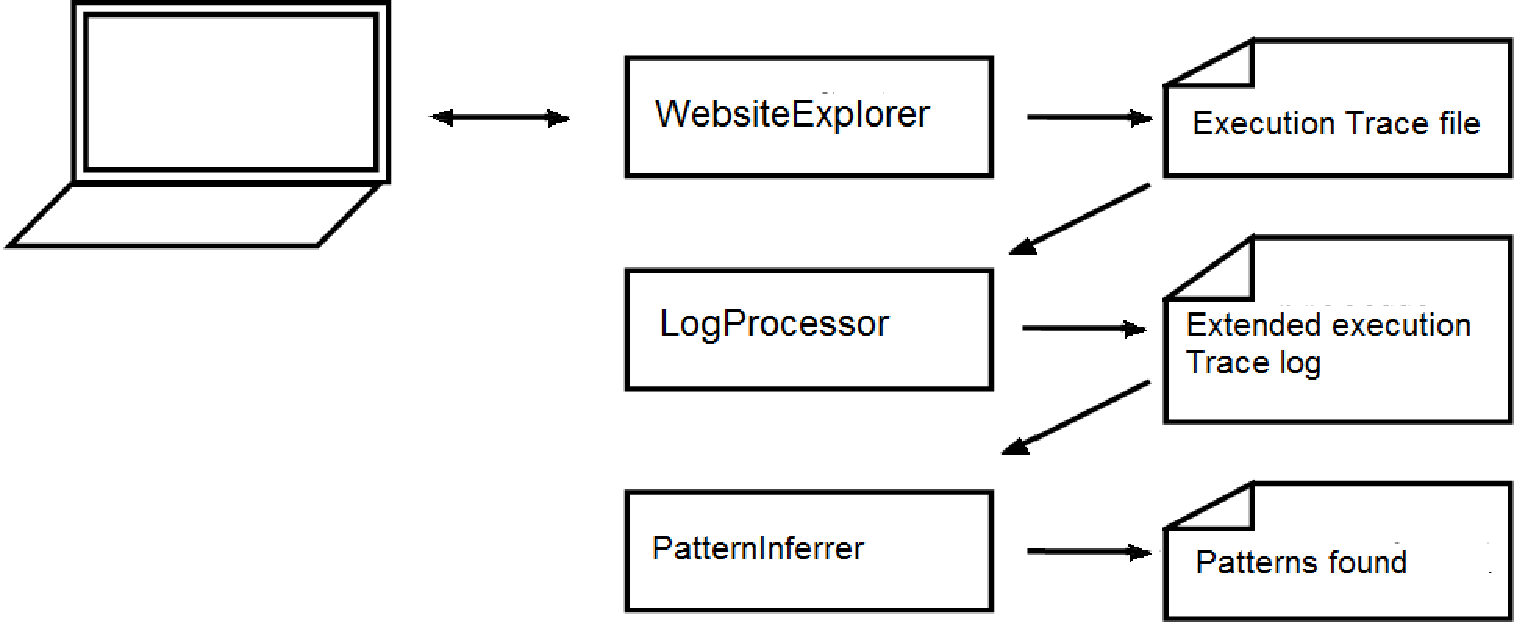
\includegraphics[scale=.3]{retool}}
%\caption{The architecture of the approach.}
%\label{fig:retool}
%\end{figure}

%A arquitectura da ferramenta pode ser vista na Figura \ref{fig:retool}. 
A abordagem pode ser dividida em três componentes: \textbf{WebsiteExplorer}, \textbf{LogProcessor}, e \textbf{PatternInferrer}.
A componente \textbf{WebsiteExplorer} carrega configurações de utilizador (que conseguem modificar quase todas as componentes da ferramenta), interage automaticamente com a aplicação e produz um ficheiro contendo o traço de execução com todas as ações tomadas. A componente \textbf{LogProcessor} é um analisador de texto, que analisa o ficheiro anterior, lê cada linha, procura por palavras-chave importantes, usa-as para identificar a ação contida na linha, e produz um ficheiro de traços de execução processado. Finalmente, a componente \textbf{PatternInferrer} analisa o último ficheiro, identifica os \textit{padrões UI}, a sua localização na página e quaisquer parâmetros existentes, e produz um ficheiro PARADIGM com os resultados, sendo as únicas exceções os padrões \textbf{Menu} e \textbf{MasterDetail}. Dado que não se pode contar que o explorador interaja com todos os elementos que pertencem a esses padrões em cada página, elementos que pertencem a esses padrões são encontrados por análise do código fonte da página e da extração de todos os elementos que obedeçam a um conjunto de regras (que podem ser mudadas através de configurações de utilizador e carregadas para a ferramenta). Os padrões identificáveis por esta ferramenta são todos os padrões de interface definidos la linguagem PARADIGM mais o padrão \textbf{Menu} (uma coleção de ligações de navegação a outras páginas Web dentro de uma página Web, geralmente organizados numa estrutura em árvore) que vai ser incluído na linguagem PARADIGM no futuro.

\section{Conclusões}\label{sec:conclui}
Esta dissertação pretende continuar o trabalho realizado na ferramenta PARADIGM-RE, uma ferramenta responsável por extrair um modelo parcial de uma aplicação Web da própria aplicação através de engenharia reversa.

A ferramenta anterior precisava que o utilizador interagisse com a aplicação para a explorar, registava a informação associada, analisava a informação guardada da interação, código fonte e URLs das páginas visitadas, e deduzia padrões através de um conjunto de regras heurísticas; a ferramenta atual é totalmente automática, requer apenas um ficheiro com o traço de execução, e deduz padrões através da análise sintática do resultado da análise lexical do ficheiro de traço de execução e, para alguns padrões, da análise do código fonte da página.

%%English version: comment first, uncomment second
\bibliographystyle{unsrt-pt}  % numeric, unsorted refs
%\bibliographystyle{unsrt}  % numeric, unsorted refs
\bibliography{myrefs}

\end{multicols}

\end{document}
